\documentclass[11pt]{article}
\usepackage[utf8]{inputenc}	% Para caracteres en español
\usepackage{amsmath,amsthm,amsfonts,amssymb,amscd}
\usepackage{multirow,booktabs}
\usepackage[table]{xcolor}
\usepackage{fullpage}
\usepackage{lastpage}
\usepackage{enumitem}
\usepackage{fancyhdr}
\usepackage{mathrsfs}
\usepackage{wrapfig}
\usepackage{setspace}
\usepackage{calc}
\usepackage{multicol}
\usepackage{cancel}
\usepackage[retainorgcmds]{IEEEtrantools}
\usepackage[margin=1cm]{geometry}
\usepackage{amsmath}
\newlength{\tabcont}
\setlength{\parindent}{0.0in}
\setlength{\parskip}{0.05in}
\usepackage{empheq}
\usepackage{framed}
\usepackage[most]{tcolorbox}
\usepackage{xcolor}
\usepackage{graphicx}
\usepackage{listings}
% -- Basic formatting
\usepackage[utf8]{inputenc}
\usepackage[english]{babel}
\usepackage{times}
\usepackage{caption}
\usepackage{subcaption}
\usepackage{placeins}
\setlength{\parindent}{0pt}
\usepackage{indentfirst}% -- Defining colors:
\usepackage[dvipsnames]{xcolor}
\definecolor{codegreen}{rgb}{0,0.6,0}
\definecolor{codegray}{rgb}{0.5,0.5,0.5}
\definecolor{codepurple}{rgb}{0.58,0,0.82}
\definecolor{backcolour}{rgb}{0.95,0.95,0.92}% Definig a custom style:
\lstdefinestyle{mystyle}{
    backgroundcolor=\color{backcolour},   
    commentstyle=\color{codepurple},
    keywordstyle=\color{NavyBlue},
    numberstyle=\tiny\color{codegray},
    stringstyle=\color{codepurple},
    basicstyle=\ttfamily\footnotesize\bfseries,
    breakatwhitespace=false,         
    breaklines=true,                 
    captionpos=t,                    
    keepspaces=true,                 
    numbers=left,                    
    numbersep=5pt,                  
    showspaces=false,                
    showstringspaces=false,
    showtabs=false,                  
    tabsize=2
}% -- Setting up the custom style:
\lstset{style=mystyle}
\lstset{
  style=mystyle,
  framexleftmargin=3.5mm,
  rulesepcolor=\color{black},
  linewidth=0.6\linewidth,
  xleftmargin=12pt,
  aboveskip=12pt,
  belowskip=12pt
}
\colorlet{shadecolor}{orange!15}
\parindent 0in
\parskip 1pt
\geometry{margin=1in, headsep=0.25in}
\theoremstyle{definition}
\newtheorem{defn}{Definition}
\newtheorem{reg}{Rule}
\newtheorem{exer}{Exercise}
\newtheorem{note}{Note}
\graphicspath{ {./images/} }
\linespread{0.75}
\begin{document}
\setcounter{section}{0}
\title{MIE223 Lecture Notes}

\thispagestyle{empty}

\begin{center}
{\LARGE \bf Introduction to Privacy and Anonymity}\\
{\large MIE223}\\
Winter 2025
\end{center}
\section{Privacy and Anonymity}

\subsection{AOL Privacy Debacle}
\begin{itemize}
    \item In August 2006, AOL released anonymized search
    query logs
    \begin{itemize}
        \item 657K users, 20M queries over 3 months
        (March-May)
    \end{itemize}
    \item Opposing goals
    \begin{itemize}
        \item Analyze data for research purposes, provide
        better services for users and advertisers
        \item Protect privacy of AOL users
        \begin{itemize}
            \item Government laws and regulations
            \item Search queries may reveal income, evaluations,
            intentions to acquire goods and services, etc.
        \end{itemize}
    \end{itemize} 
\end{itemize}

\subsection{AOL User 4417749}
\begin{itemize}
    \item AOL query logs have the form
    <AnonID, Query, QueryTime, ItemRank, ClickURL>
    \begin{itemize}
        \item ClickURL is the truncated URL
    \end{itemize} 
    \item NY Times re-identified AnonID 4417749
    \begin{itemize}
        \item Sample queries: “numb fingers”, “60 single men”,
        “dog that urinates on everything”, “landscapers
        in Lilburn, GA”, several people with the last
        name Arnold
        \begin{itemize}
            \item Lilburn area has only 14 citizens with the last
            name Arnold
        \end{itemize}
        \item NYT contacts the 14 citizens, finds out AOL User
        4417749 is 62-year-old Thelma Arnold
    \end{itemize}
\end{itemize}

\subsection{Foundations of Privacy}
\begin{itemize}
    \item Consent:
    \begin{itemize}
        \item GDPR (EU), US (Privacy Act of 1974)
    \end{itemize} 
    \item Notice: you have to accept collection practices
    \begin{itemize}
        \item Question: who are some of the major providers of user web data?
    \end{itemize}
    \item De-identification
    \begin{itemize}
        \item Only release attributes that could not identify you
        \item Historically founded on principle of k-anonymity
        \begin{itemize}
            \item Re-identification: multiple attributes can as well as quasi-
            identifiers (partial postal code) that link you accross datasets
            (medical, voter) even with k-anonymity
            \begin{itemize}
                \item Sweeney (Harvard) used 1990 Census data to estimate that 0.04
                percent of the United States population was uniquely identified
                by the basic demographic fields allowed by the HIPAA Safe
                Harbor – namely, year of birth, gender, and first 3 digits of ZIP
            \end{itemize}
        \end{itemize}
    \end{itemize}
\end{itemize}

\subsection{Background}
\begin{itemize}
    \item Large amount of person-specific data has been
    collected in recent years
    \begin{itemize}
        \item Both by governments and by private entities
    \end{itemize}
    \item Data and knowledge extracted by data mining
    techniques represent a key asset to the society
    \begin{itemize}
        \item Analyzing trends and patterns
        \item Formulating public policies
    \end{itemize}
    \item Laws and regulations require that some collected
    data must be made public
    \begin{itemize}
        \item For example, Census data
    \end{itemize}
\end{itemize}

\subsection{Public Data Conundrum}
\begin{itemize}
    \item Health-care datasets
    \begin{itemize}
        \item Clinical studies, hospital discharge databases
    \end{itemize}
    \item Genetic datasets
    \begin{itemize}
        \item \$1000 genome, HapMap, deCode
    \end{itemize}
    \item Demographic datasets
    \begin{itemize}
        \item U.S. Census Bureau, sociology studies
    \end{itemize}
    \item Search logs, recommender systems, social networks, blogs
    \begin{itemize}
        \item AOL search data, social networks of blogging sites, Netflix movie ratings, Amazon
    \end{itemize}
\end{itemize}

\subsection{What About Privacy?}
\begin{itemize}
    \item First thought: anonymize the data
    \item How?
    \item Remove “personally identifying information” (PII)
    \begin{itemize}
        \item Name, Social Security number, phone number, email, address... what else?
        \item Anything that identifies the person directly
    \end{itemize}
    \item Is this enough? No!
\end{itemize}

\subsection{Re-identification by Linking}
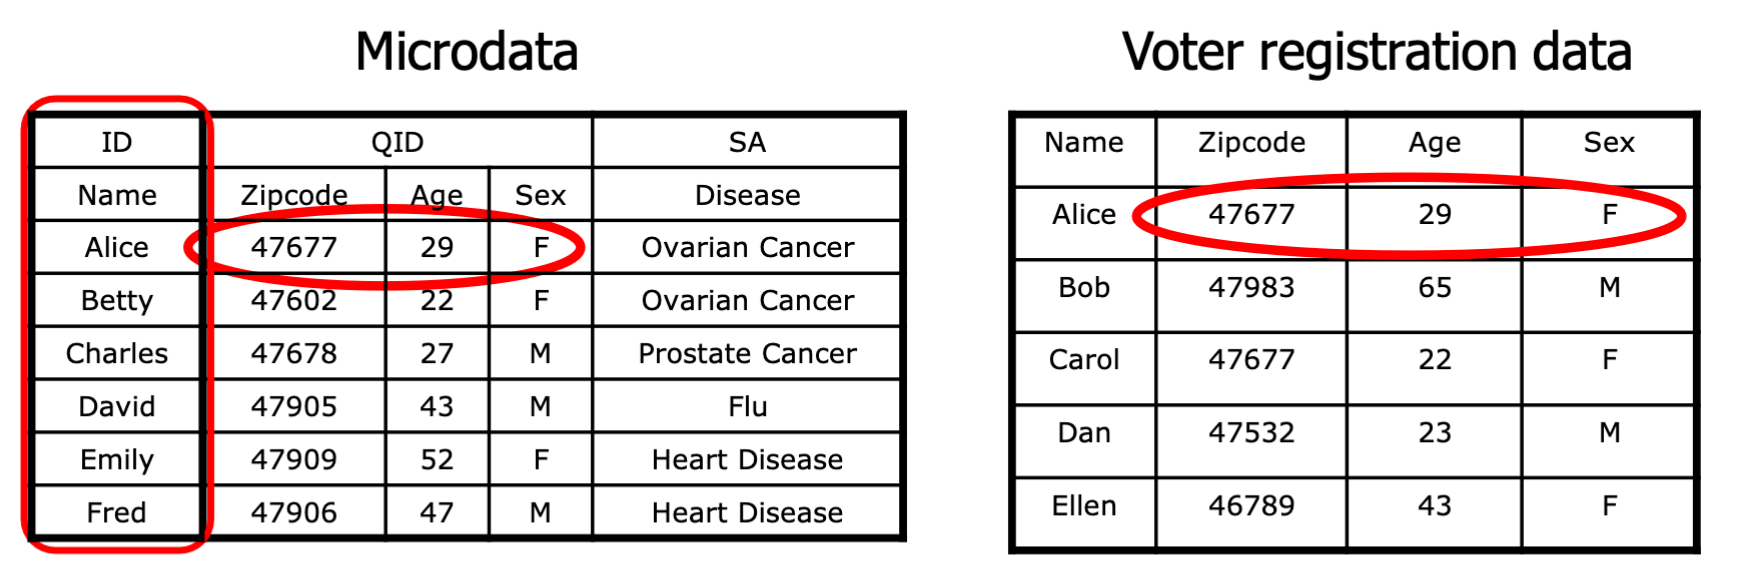
\includegraphics[width=\textwidth/2]{14.png}

ID is the PII, the rest isn't. When combined they are quasi-identifiers

Voter registration data is all PII.

\subsection{Latanya Sweeney’s Attack (1997)}
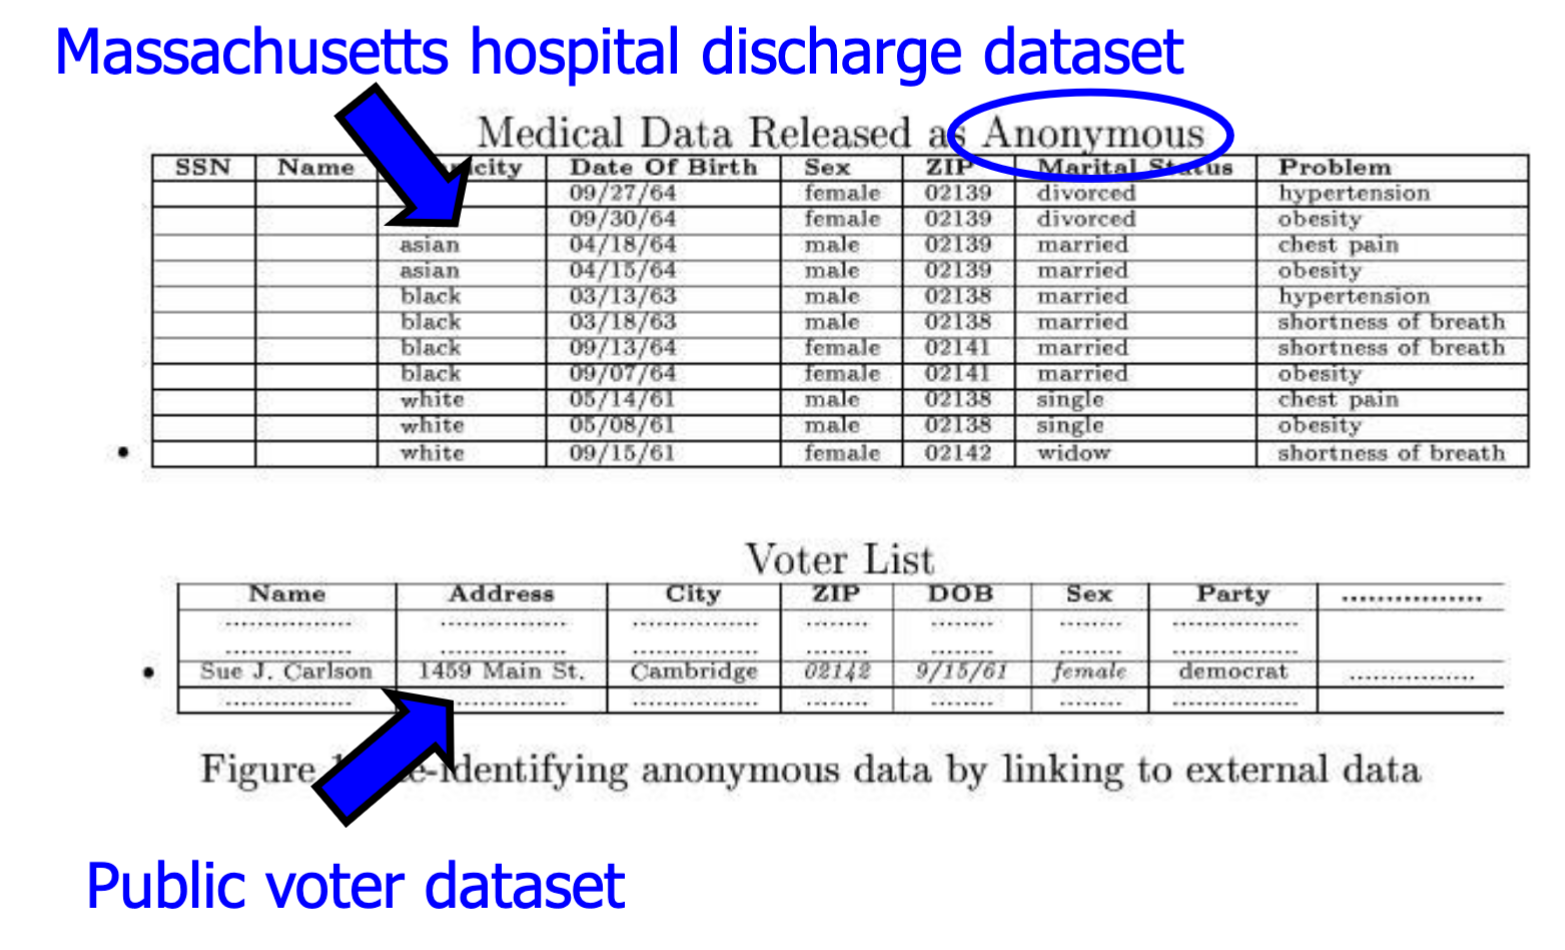
\includegraphics[width=\textwidth/2]{15.png}

\subsection{Quasi-Identifiers}
\begin{itemize}
    \item Key attributes
    \begin{itemize}
        \item Name, address, phone number - uniquely identifying!
        \item Always removed before release
    \end{itemize}
    \item Quasi-identifiers
    \begin{itemize}
        \item (5-digit ZIP code, birth date, gender) uniquely identify 87\% of the population in the U.S.
        \item Can be used for linking anonymized dataset with other datasets
    \end{itemize}
\end{itemize}

\subsection{Classification of Attributes}
\begin{itemize}
    \item Sensitive attributes
    \begin{itemize}
        \item Medical records, salaries, etc.
        \item These attributes are what the researchers need, so they are always released directly
    \end{itemize}
\end{itemize}
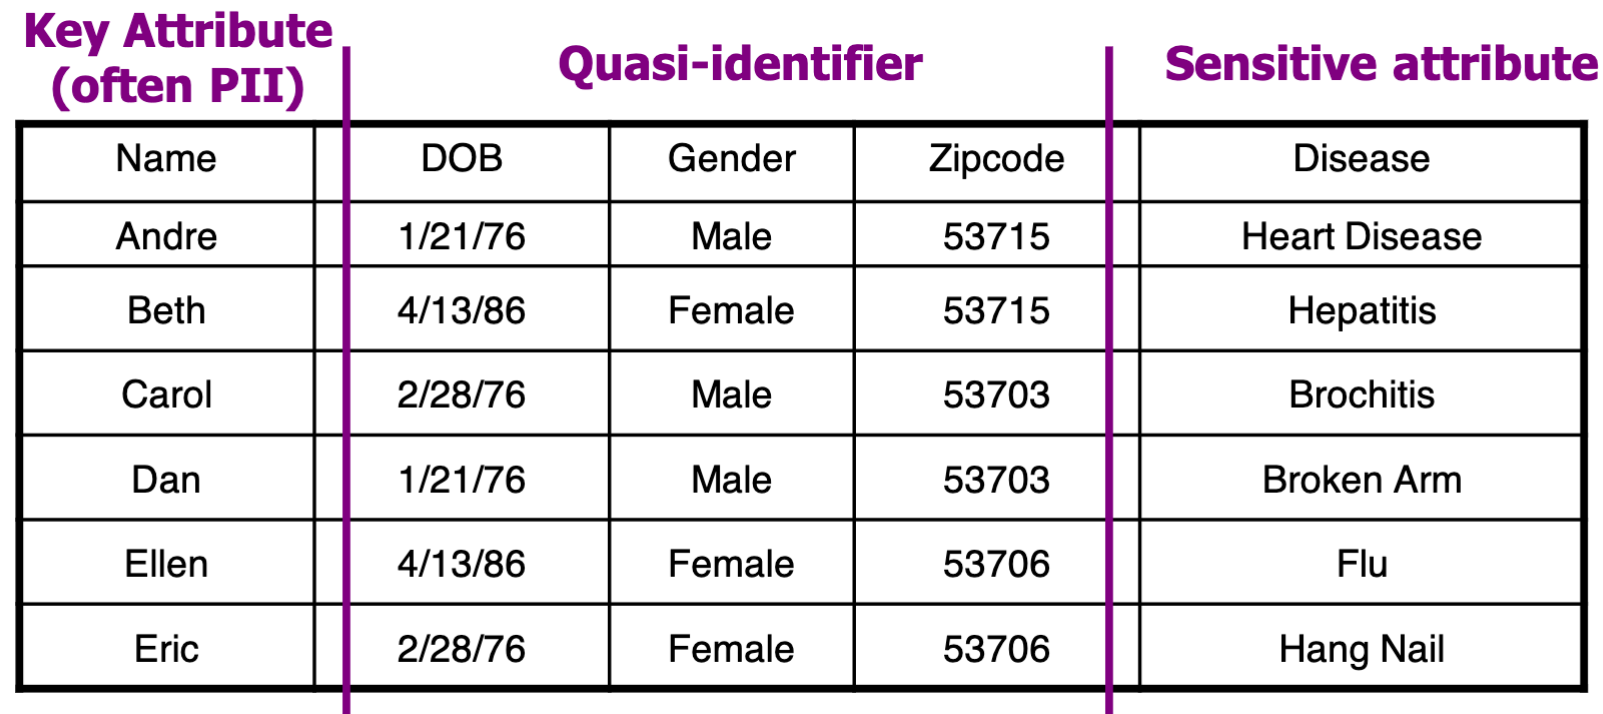
\includegraphics[width=\textwidth/2]{16.png}

\subsection{K-Anonymity: Intuition}
\begin{itemize}
    \item The information for each person contained in the released table cannot be distinguished from at least k-1 individuals whose information also appears in the release
    \begin{itemize}
        \item Example: you try to identify a man in the released table, but the only information you have is his birth date and gender. There are k men in the table with the same birth date and gender.
    \end{itemize}
    \item Any quasi-identifier present in the released table must appear in at least k records
\end{itemize}

\subsection{k-Anonymity via Generalization}
\begin{itemize}
    \item Goal of k-Anonymity
    \begin{itemize}
        \item Each record is indistinguishable from at least k-1 other records
        \item These k records form an equivalence class
    \end{itemize}
    \item Generalization: replace quasi-identifiers with less specific, but semantically consistent values
    \item If you just drop rows if not k-anonymous you cause missingness not at random
    \item you want to avoid dropping rows to avoid changing decisions, you can just generate attributes instead
    \item Example: replace 5-digit ZIP code with 3-digit ZIP code
\end{itemize}
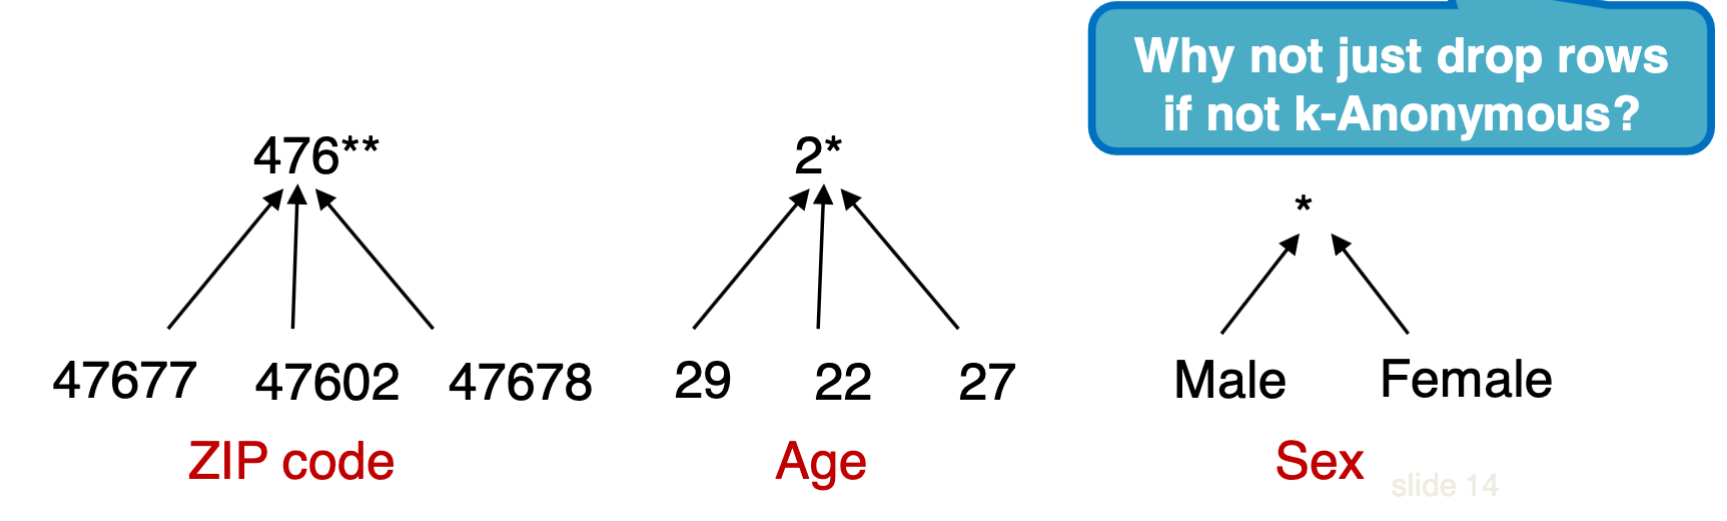
\includegraphics[width=\textwidth/2]{17.png}

\subsection{Achieving k-Anonymity}
\begin{itemize}
    \item Generalization
    \begin{itemize}
        \item Replace specific quasi-identifiers with less specific values until get k identical values
        \item Partition ordered-value domains into intervals
    \end{itemize}
    \item Problem: Suppression
    \begin{itemize}
        \item When generalization causes too much information loss
        \item This is common with “outliers”
    \end{itemize}
    \item Lots of algorithms in the literature
    \begin{itemize}
        \item Aim to produce “useful” anonymizations
        \item ... usually without any clear notion of utility
    \end{itemize}
\end{itemize}

\subsection{Example of a k-Anonymous Table}
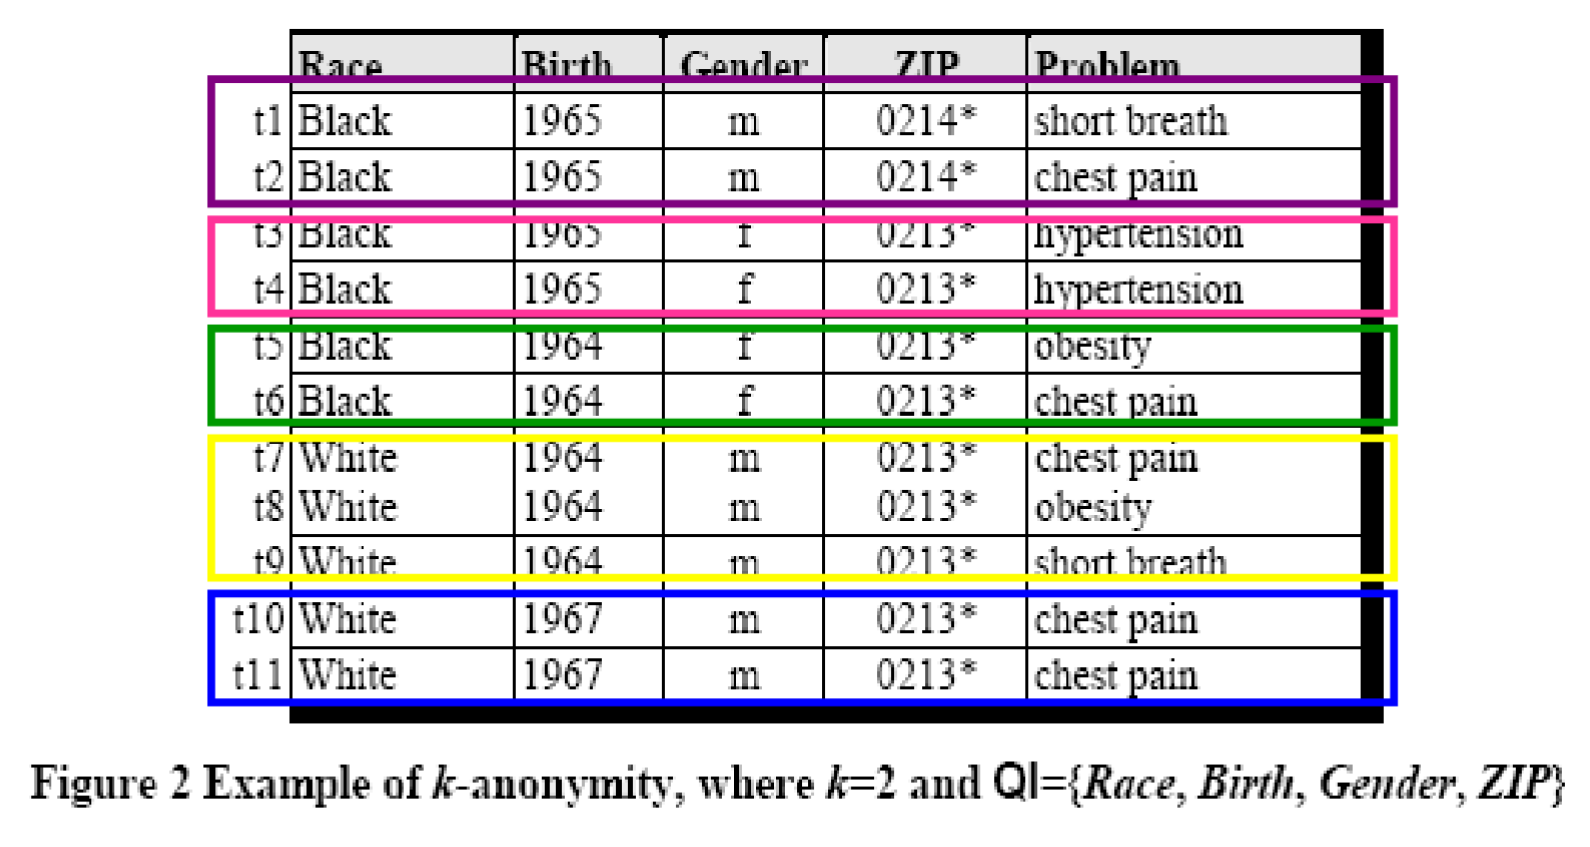
\includegraphics[width=\textwidth/2]{18.png}

k = 2 and not k = 3 because we take the lowest k value.

\subsection{Example of Generalization (1)}
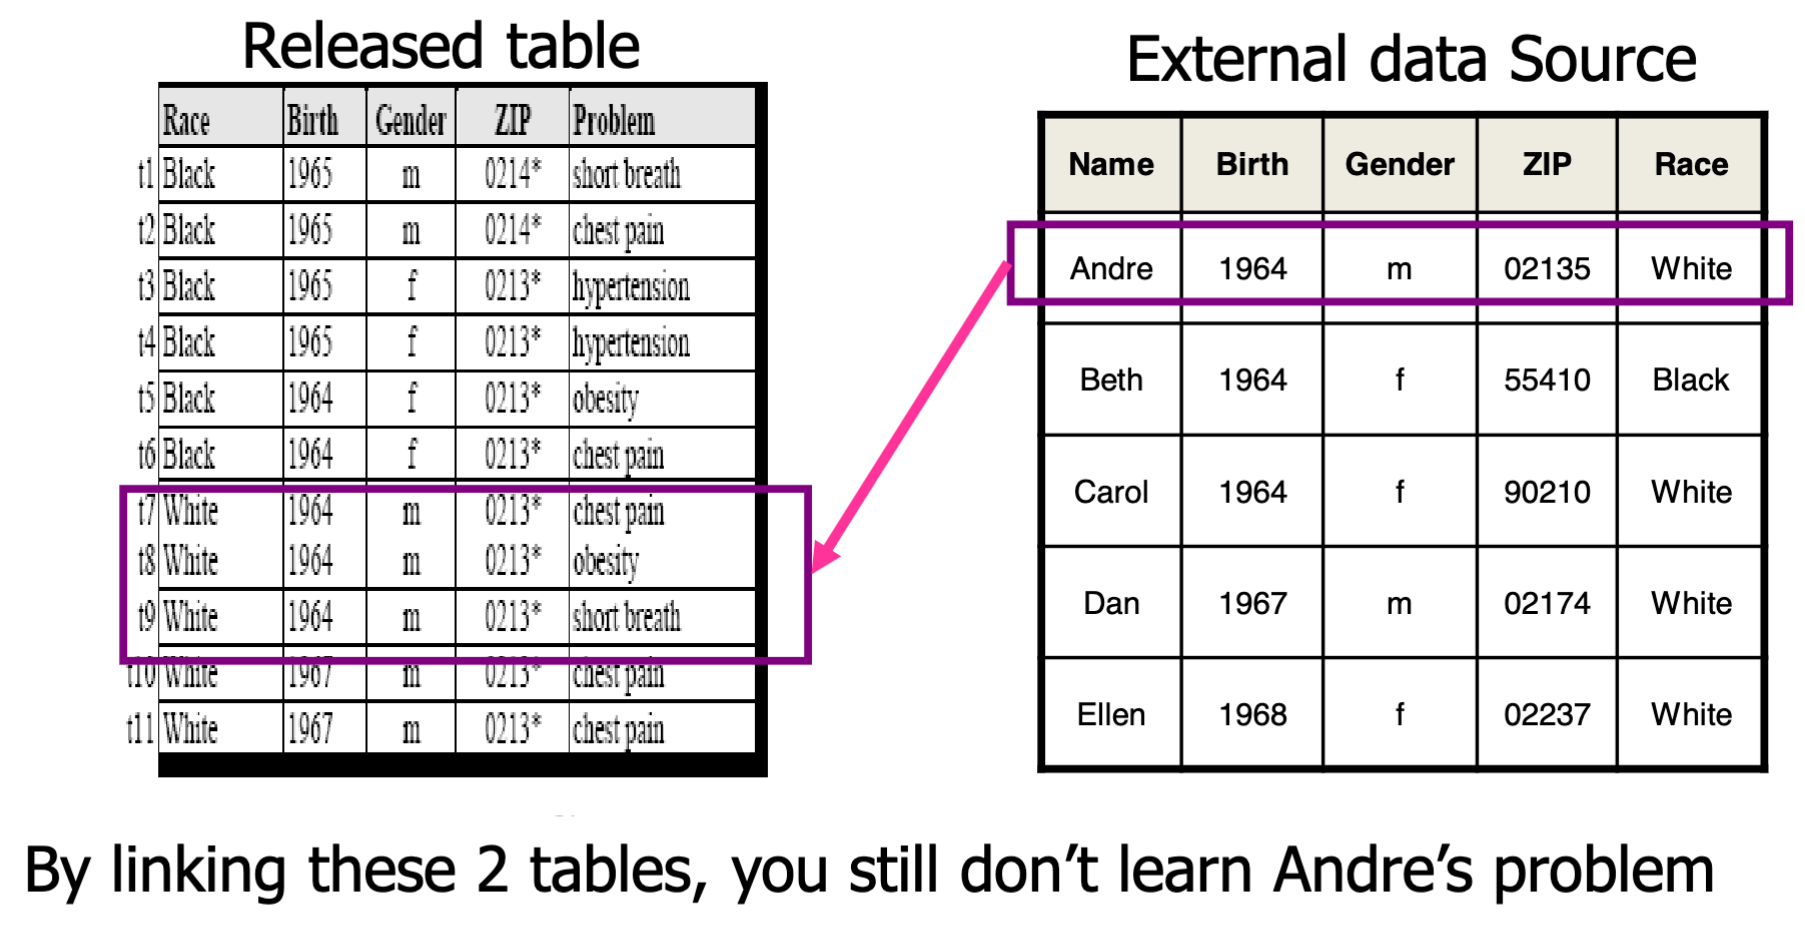
\includegraphics[width=\textwidth/2]{19.png}

\subsection{Example of Generalization (2)}
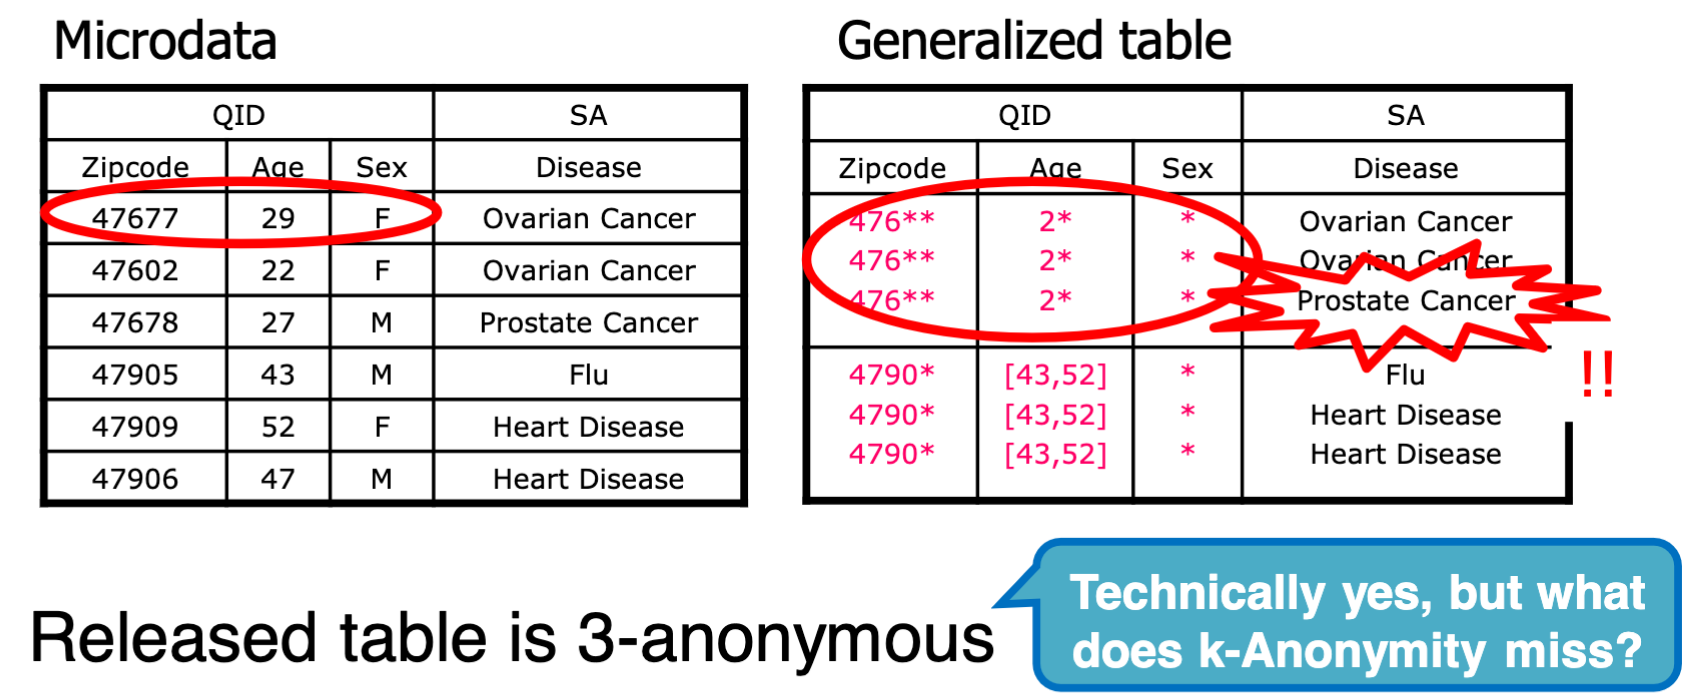
\includegraphics[width=\textwidth/2]{20.png}

If the adversary knows Alice’s quasi-identifier
(47677, 29, F), they still do not know which of the
first 3 records corresponds to Alice’s record

\subsection{Curse of Dimensionality}
\begin{itemize}
    \item Generalization fundamentally relies on locality of quasi-identifiers
    \begin{itemize}
        \item Each record must have k close neighbors
    \end{itemize}
    \item Real-world datasets are very sparse
    \begin{itemize}
        \item Many attributes (dimensions)
        \begin{itemize}
            \item Netflix Prize dataset: 17,000 dimensions
            \item Amazon customer records: several million dimensions
        \end{itemize}
        \item “Nearest neighbor” is very far
    \end{itemize}
    \item Projection to low dimensions loses all info
    \begin{itemize}
        \item k-anonymized datasets are useless
    \end{itemize}
\end{itemize}

\subsection{HIPAA Privacy Rule (US)}
"Under the safe harbor method, covered entities must remove all of a
list of 18 enumerated identifiers and have no actual knowledge that
the information remaining could be used, alone or in combination, to
identify a subject of the information."

“The identifiers that must be removed include direct identifiers, such
as name, street address, social security number, as well as other
identifiers, such as birth date, admission and discharge dates, and
five-digit zip code. The safe harbor requires removal of geographic
subdivisions smaller than a State, except for the initial three digits of a
zip code if the geographic unit formed by combining all zip codes with
the same initial three digits contains more than 20,000 people. In
addition, age, if less than 90, gender, ethnicity, and other demographic
information not listed may remain in the information. The safe harbor
is intended to provide covered entities with a simple, definitive method
that does not require much judgment by the covered entity to
determine if the information is adequately de-identified."

\subsection{Two (and a Half) Interpretations}
\begin{enumerate}
    \item Membership disclosure: Attacker cannot tell that a
    given person in the dataset
    \item Sensitive attribute disclosure: Attacker cannot tell
    that a given person has a certain sensitive
    attribute
    \item Identity disclosure: Attacker cannot tell which
    record corresponds to a given person
\end{enumerate}

This (3) interpretation is correct, assuming the attacker
does not know anything other than quasi-identifiers
But this does not imply any privacy!
Example: k clinical records, all HIV+

\subsection{Attacks on k-Anonymity}
\begin{itemize}
    \item k-Anonymity does not provide privacy if
    \begin{itemize}
        \item Sensitive values in an equivalence class lack diversity
        \item The attacker has background knowledge
    \end{itemize}
\end{itemize}

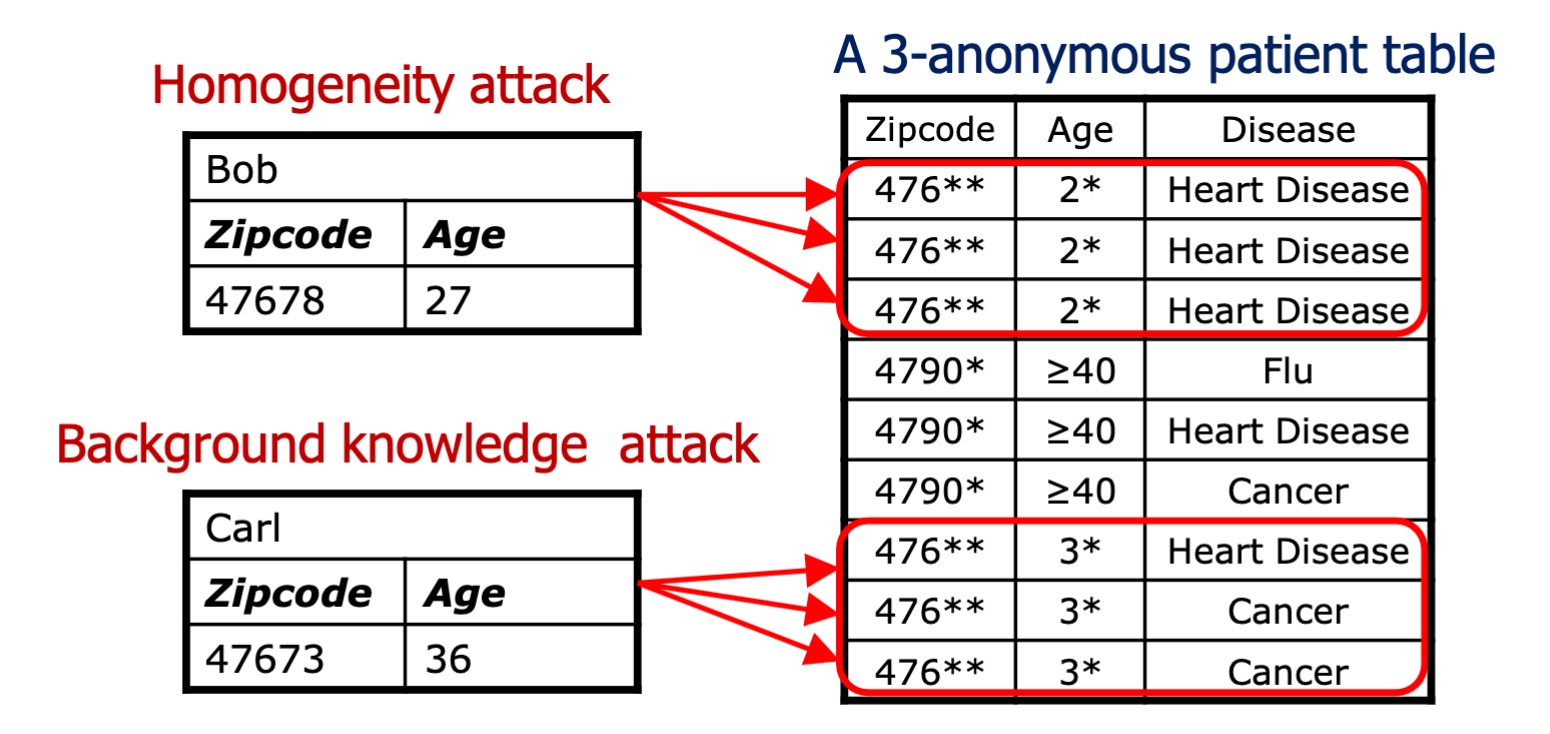
\includegraphics[width=\textwidth/2]{21.png}

\subsection{l-Diversity}
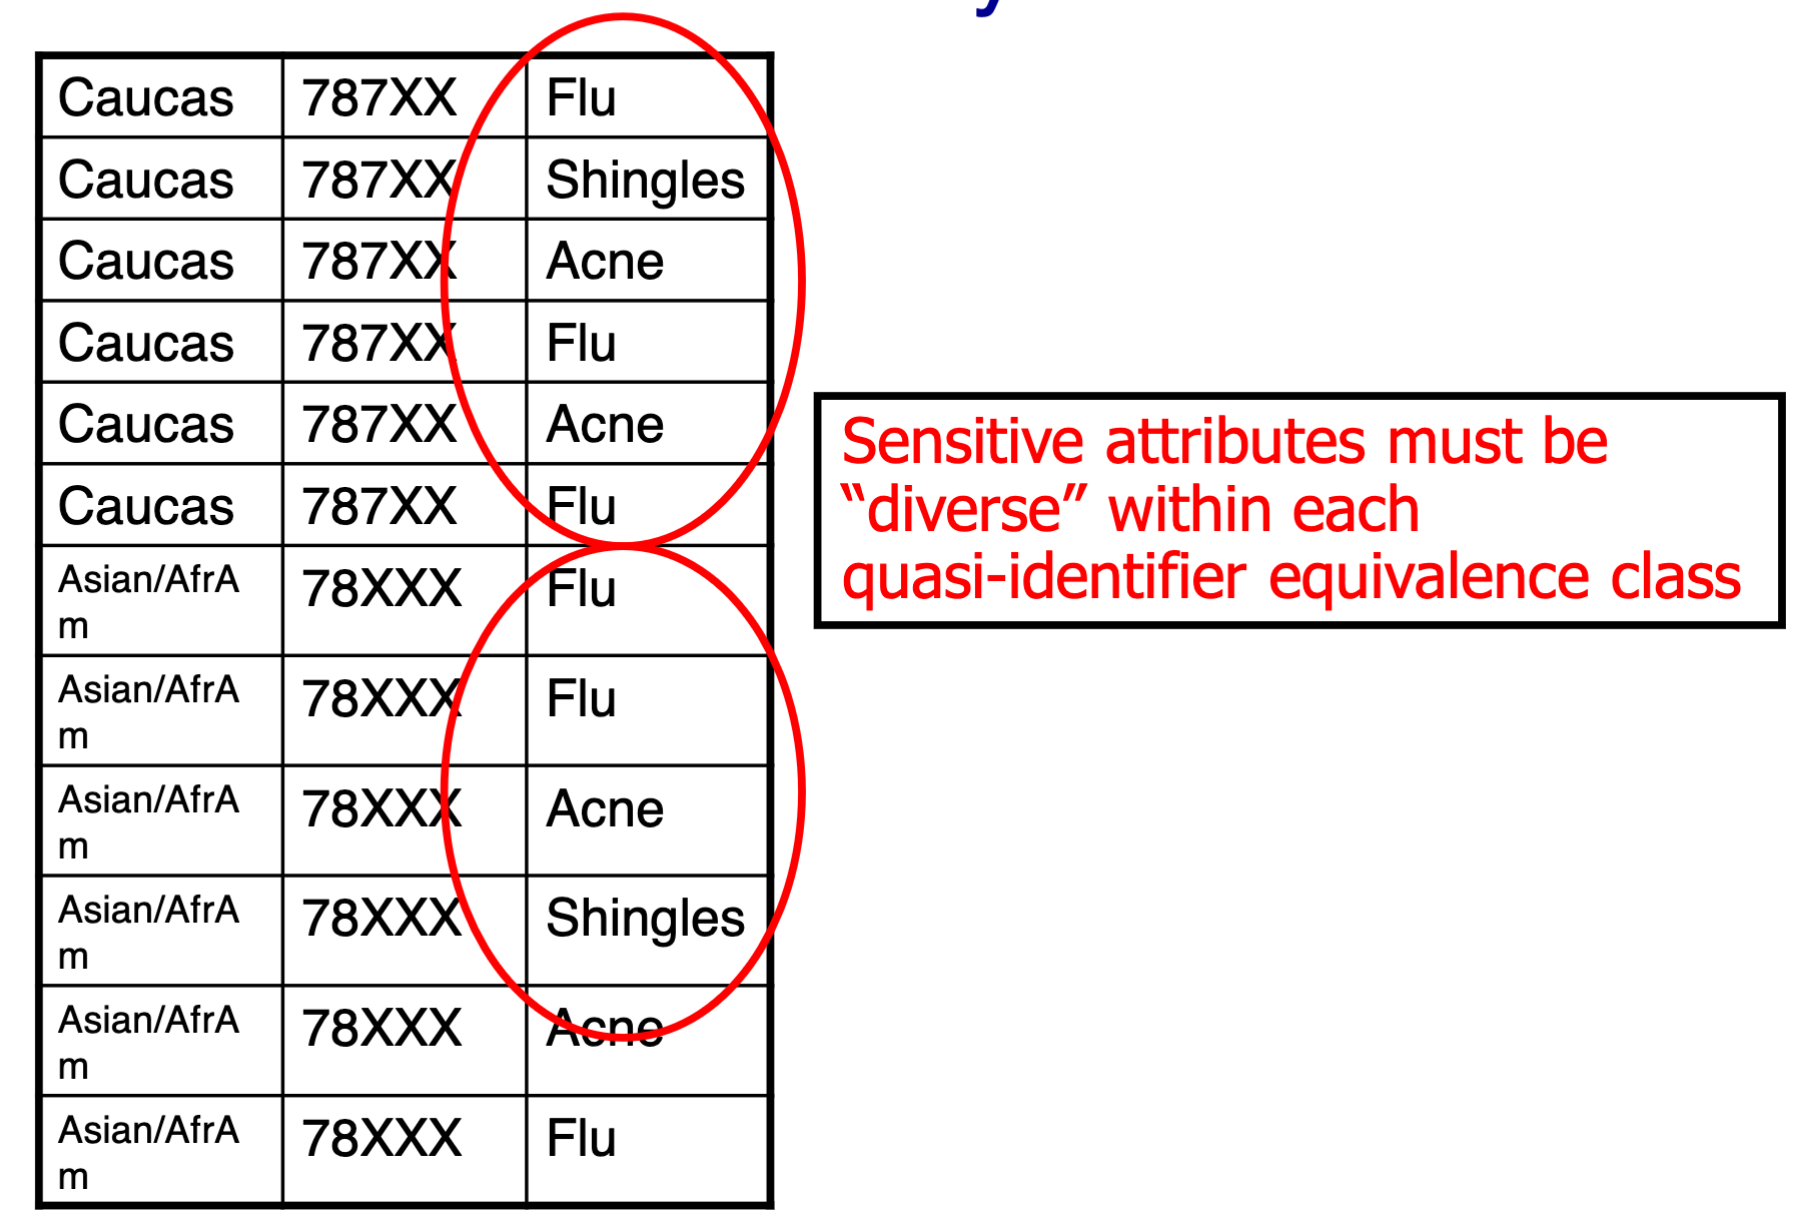
\includegraphics[width=\textwidth/2]{22.png}

\subsection{Distinct l-Diversity}
\begin{itemize}
    \item Each equivalence class of quasi-identifiers has at
    least l well-represented sensitive values
    \item Doesn’t prevent probabilistic inference attacks
\end{itemize}
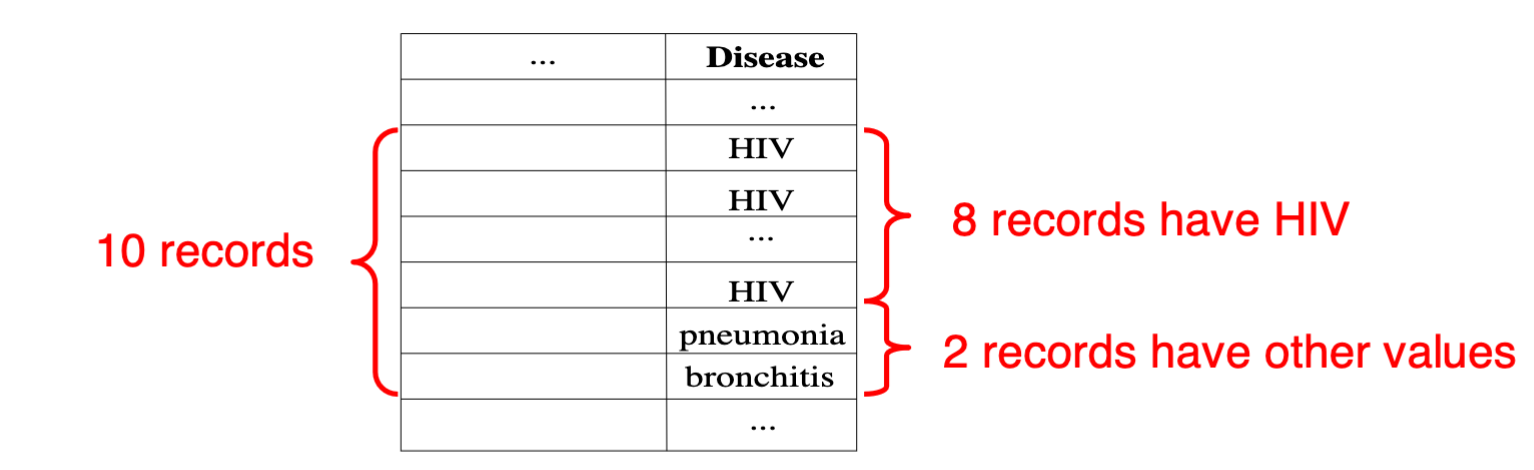
\includegraphics[width=\textwidth/2]{23.png}

I = 10\% here. 

\subsection{Other Versions of l-Diversity}
\begin{itemize}
    \item Probabilistic l-diversity
    \begin{itemize}
        \item The frequency of the most frequent value in an equivalence class is bounded by 1/l
    \end{itemize}
    \item Entropy l-diversity
    \begin{itemize}
        \item The entropy of the distribution of sensitive values in each equivalence class is at least log(l)
    \end{itemize}
    \item Recursive (c,l)-diversity
    \begin{itemize}
        \item \( r_1 < c(r_l + r_{l+1} + \dots + r_m) \), where \( r_i \) is the frequency of the \( i \)-th most frequent value
        \item Intuition: the most frequent value does not appear too frequently
    \end{itemize}
\end{itemize}

\subsection{t-Closeness} 
(not tested)
Distribution of sensitive
attributes within each
quasi-identifier group should
be “close” to their distribution
in the entire original database

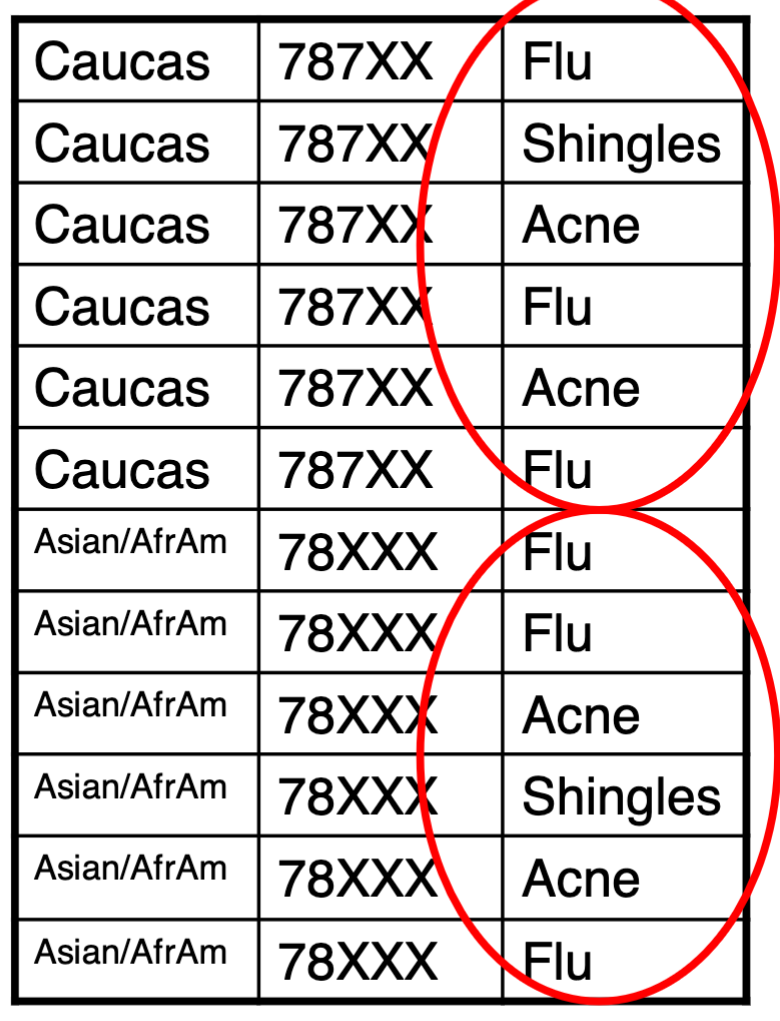
\includegraphics[width=\textwidth/4]{24.png}

\subsection{Anonymous, “t-Close” Dataset}
This is k-anonymous,
l-diverse and t-close...
...so secure, right?

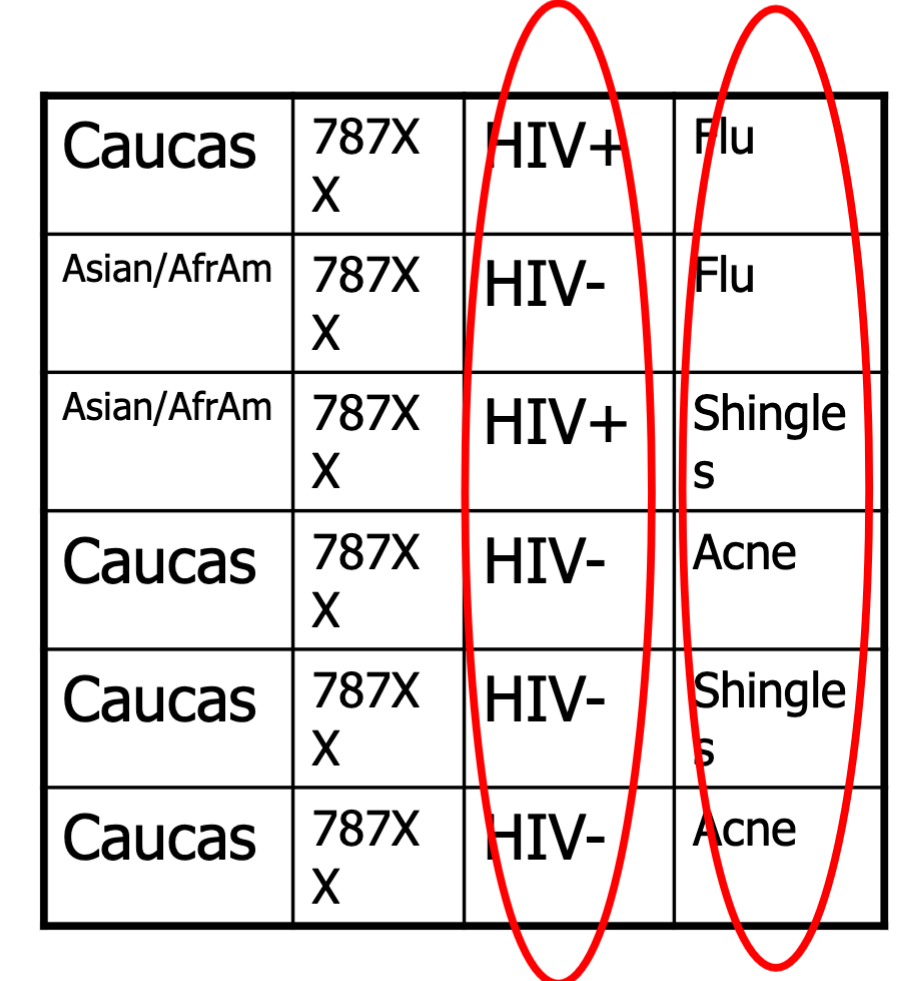
\includegraphics[width=\textwidth/3]{25.png}

\subsection{What Does Attacker Know?}
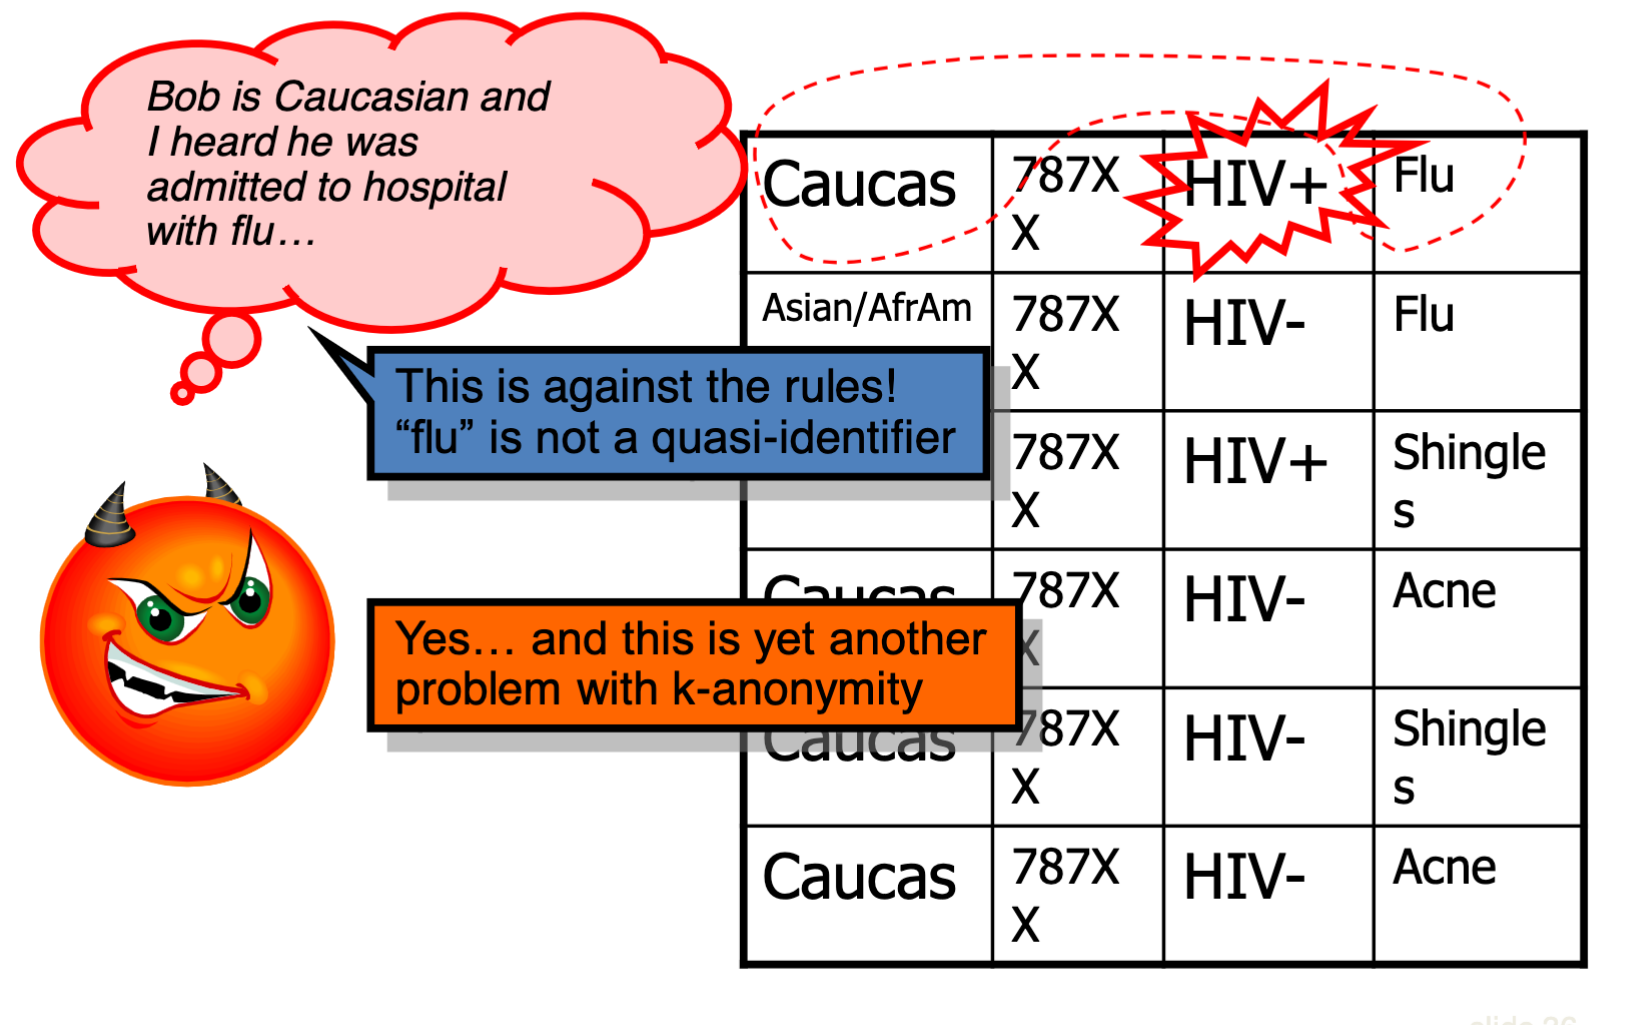
\includegraphics[width=\textwidth/3]{26.png}

\subsection{k-Anonymity is Not Enough!}
\begin{itemize}
    \item Syntactic
    \begin{itemize}
        \item Focuses on data transformation, not on what can be learned from the anonymized dataset
        \item “k-anonymous” dataset can leak sensitive information
    \end{itemize}
    \item “Quasi-identifier” fallacy
    \begin{itemize}
        \item Assumes a priori that attacker will not know certain information about their target
    \end{itemize}
    \item Can increase levels of anonymity, but ...
    \begin{itemize}
        \item Destroys utility of many real-world datasets
    \end{itemize}
\end{itemize}

\subsection{Exam question}
How can you attack a k-anonymous dataset?

\end{document}